% file: 3-1-dp/optimal-bst.tex

\documentclass[tikz]{standalone}
\usepackage{tikz-qtree}

\newcommand{\lnode}[3]{\node [label = {#1} : {$#2$}] {#3};}

\begin{document}
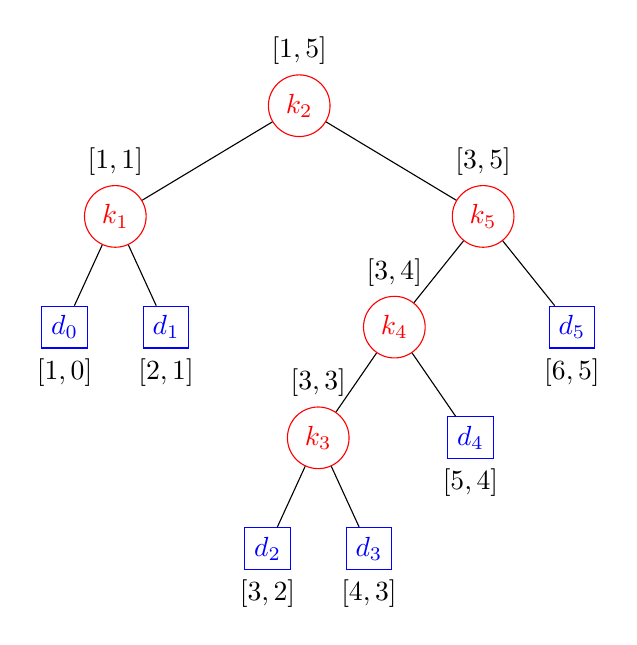
\begin{tikzpicture}[level distance = 40pt, sibling distance = 10pt,
  edge from parent/.style= {
  	draw, edge from parent path={(\tikzparentnode) -- (\tikzchildnode)}}]
  \tikzset{every internal node/.style = {draw, circle, red}}
  \tikzset{every leaf node/.style = {draw, rectangle, blue}}

  % \lnode{above}{[1,5]}{$k_2$} 

  \Tree [.\node[label = above : {$[1,5]$}]{$k_2$}; 
	  [.\node[label = above : {$[1,1]$}] {$k_1$}; 
	    \node[label = below : {$[1,0]$}] {$d_0$};
	    \node[label = below : {$[2,1]$}] {$d_1$};
	  ] 
	  [.\node[label = above : {$[3,5]$}] {$k_5$};
	    [.\node[label = above : {$[3,4]$}] {$k_4$};
	      [.\node[label = above : {$[3,3]$}] {$k_3$}; 
		\node[label = below : {$[3,2]$}] {$d_2$};
		\node[label = below : {$[4,3]$}] {$d_3$};
	      ]
	      \node[label = below : {$[5,4]$}] {$d_4$};
	    ]
	    \node[label = below : {$[6,5]$}] {$d_5$};
	  ]
	]
\end{tikzpicture}
\end{document}